\documentclass[lang=cn,newtx,12pt,scheme=chinese]{elegantbook}
\usepackage{graphicx}
\usepackage{float}
\usepackage{booktabs}

\title{《数值分析B》笔记、习题与实验}

\author{Chad Holton}
\institute{哈尔滨工业大学能源科学与工程学院}
\date{\today}
\bioinfo{邮箱}{chadholton@qq.com}
\setcounter{tocdepth}{3}

\cover{cover.png}

% 本文档命令
\usepackage{array}
\newcommand{\ccr}[1]{\makecell{{\color{#1}\rule{1cm}{1cm}}}}

% 修改标题页的色带
\definecolor{customcolor}{RGB}{32,128,150}
\colorlet{coverlinecolor}{customcolor}
\usepackage{cprotect}

\begin{document}

\maketitle
\frontmatter

\tableofcontents

\mainmatter
\chapter*{前言}
《数值分析》是许多专业的研究生阶段的必修科目, 本文档是我学习整理的笔记、习题和实验部分,适用于哈尔滨工业大学的数值分析B课程.本科数学例如高数的大一和考研的题型与难度也不一样.高等数学因为存在考研所以内容规范且稳定,而数值分析每个学校内容重点都不同.2025级32课时+4次上机实验,很多内容比较简略,话说是不是压缩课时了,讲真教材、PPT与习题需要相应更新以适应压缩课时的情形.你问下AI让它设计32学时的授课方案,它认为课时有限会删很多东西.\LaTeX 源代码在本人的GitHub主页\href{https://github.com/phychi}{phychi}, 虽然也没有什么内容.本文档部分内容可能有些刻意,不像笔记.

感谢\href{https://github.com/ElegantLaTeX}{ElegantLaTeX}提供的精美模板,停止更新太可惜了.
\chapter{绪论}
数值计算的根本任务是研究算法. 计算机基础运算是加减乘除, 其他计算转化为这, 根据步数等衡量算法的优劣.
\begin{itemize}
	\item 计算$\sin x$, 可以用泰勒公式展开$\sin x=x-\dfrac{x^3}{3!}+\dfrac{x^5}{5!}\cdots(-1)^n\dfrac{x^{2n+1}}{(2n+1)!}+R_{2n+1}(x)$取前几项近似.
	\item 解线性方程组有Cramer法则, 但是按照这个方法, 计算$n$阶行列式的值如果按照定义, 随着$n$的增加, 计算量会极速增长, 需要更好的算法.
\end{itemize}
\section{误差的定义}
\textbf{误差}, 即一个物理量的真实值与计算值之间的差异, 来源可以分为四类.
\begin{itemize}
	\item 从实际问题中抽象出数学模型, 即\textbf{模型误差}. 例如在建模时的非线性模型的线性化.
	\item 通过\textbf{测量}得到模型中参数的值, 即\textbf{观测误差}.
	\item 求近似解, 展开取前几项, 即\textbf{截断误差}.
	\item 机器字长有限, 保留几位有效数字, 即\textbf{舍入误差}.
\end{itemize}
如下图, 泰勒展开取前4项, 剩余项即截断误差, 而前四项求和有两项要小数四舍五入的舍入误差.
\begin{figure}[H]
	\centering
	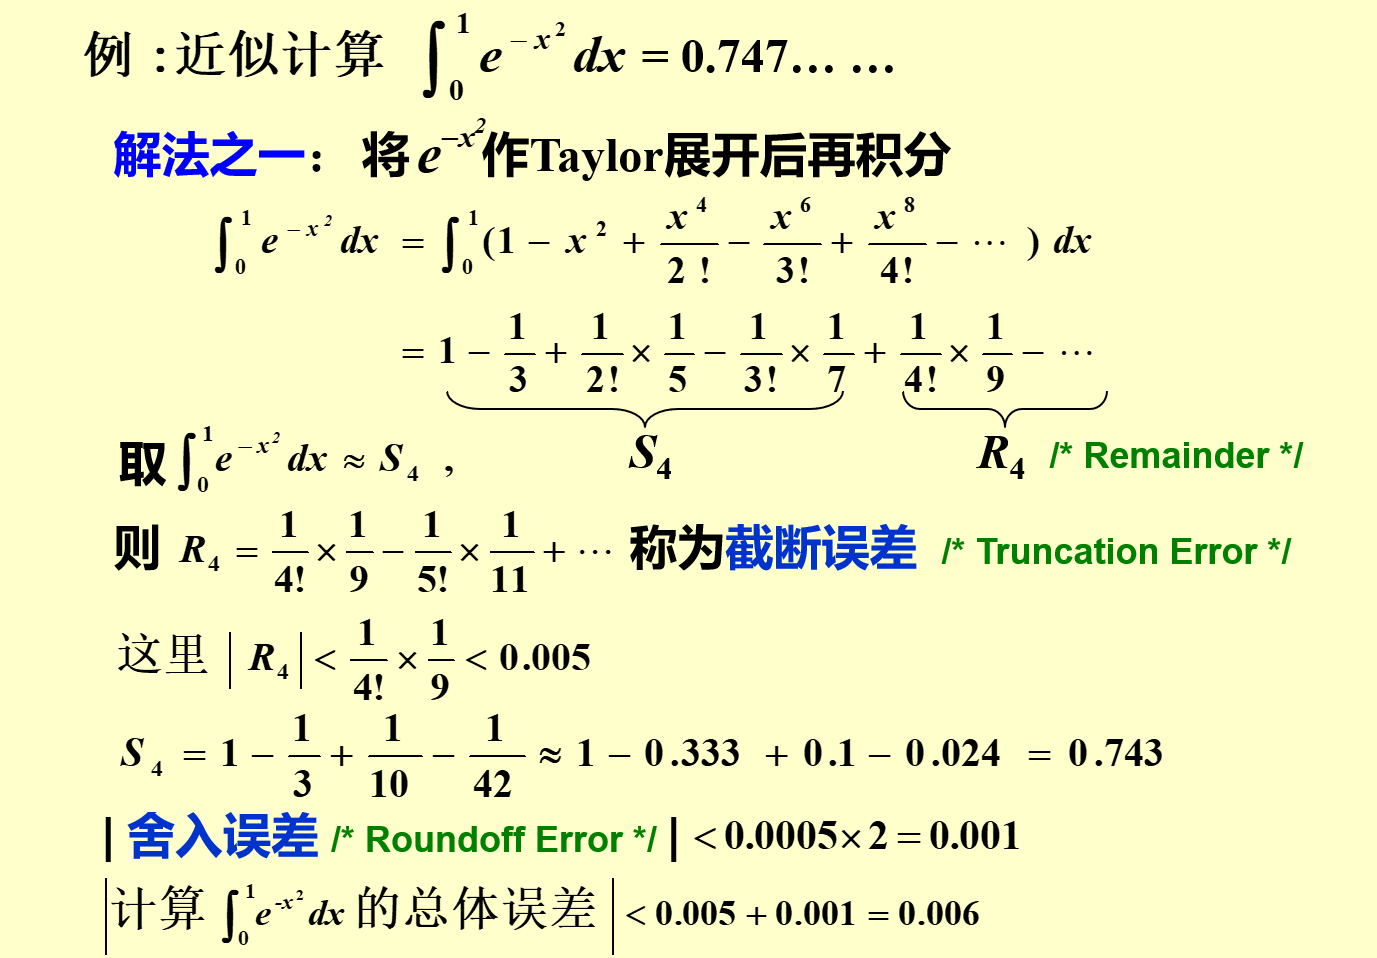
\includegraphics[width=0.9\linewidth]{image/误差1}
	\caption{误差举例}
	\label{fig:1}
\end{figure}
\section{一个算法稳定性的例子}
\begin{definition}
	一个算法如果输入数据有误差, 而在计算过程中舍入误差不增长, 则称此算法是稳定的; 否则称此算法是不稳定的.
\end{definition}
\begin{example}
	计算$I_n=e^{-1}\int_{0}^{1}x^ne^x$并估计误差.
\end{example}
存在两种计算方法, 对比效果.

公式一: $I_n=1-nI_{n-1}$, 可以看到随着$n$增长计算结果越来越离谱.
\begin{figure}[H]
	\centering
	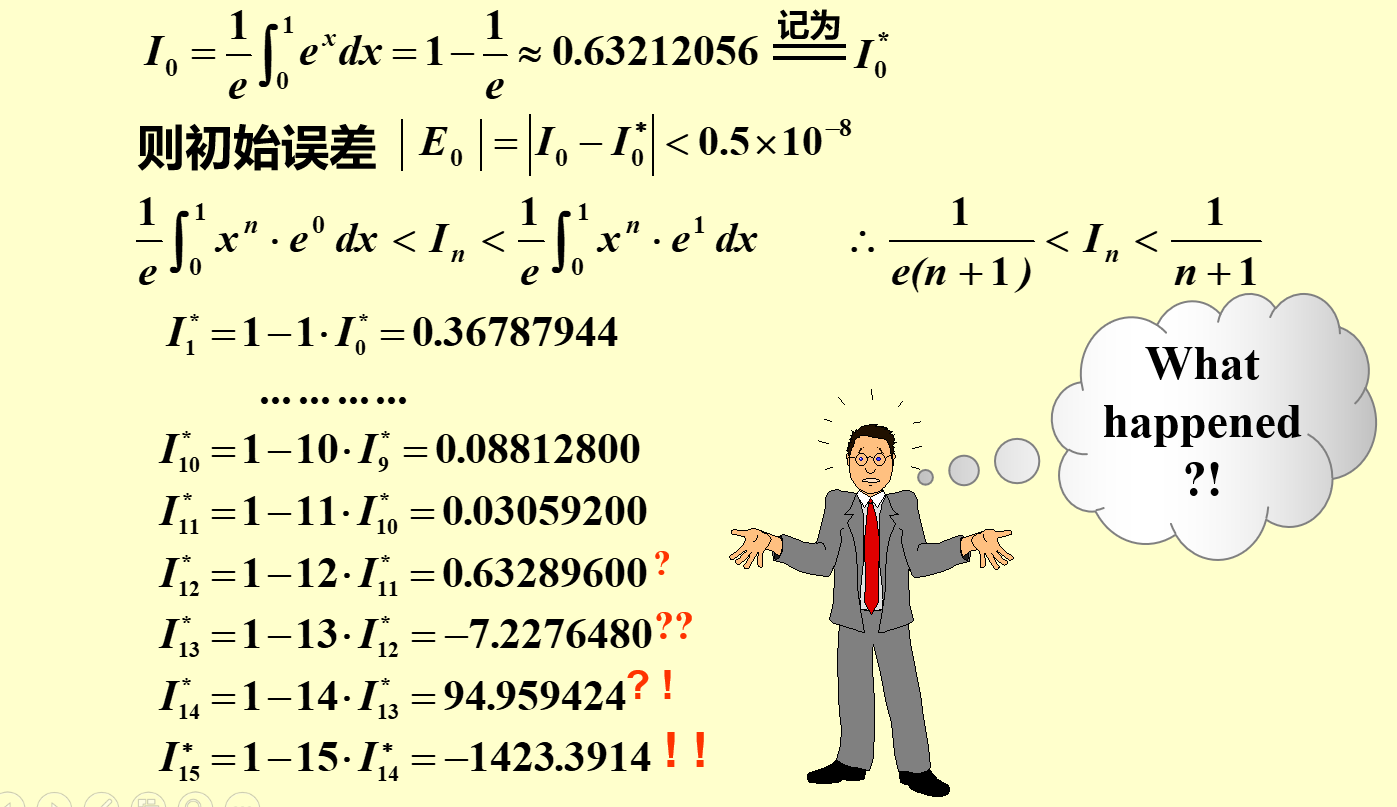
\includegraphics[width=0.7\linewidth]{image/误差2}
	\caption{不稳定算法}
	\label{fig:2}
\end{figure}
根据递推式$|E_n|=|I_n-I_n^*|=n|E_{n-1}|=\cdots=n!|E_0| $, 可见初始的小扰动$|E_0|<0.5\times10^{-8}$迅速积累,误差快速增长, 这是不稳定的算法 

公式二: $I_{n-1}=\dfrac{1}{n}(1-I_n)$, 先估计一个$I_N$ ,再反推要求的$I_n(n << N )$. 可取\[ 
I_N^*=\dfrac{1}{2}[\dfrac{1}{e(N+1)}+\dfrac{1}{N+1}]\approx I_N
 \]
 
 当$N\to+\infty$时, $|E_N|=|I_N-I_N^*|\to0$, 其绝对误差很小, 但相对误差可能比较大, 使用该方法理由后面会知道.
 \begin{figure}[H]
 	\centering
 	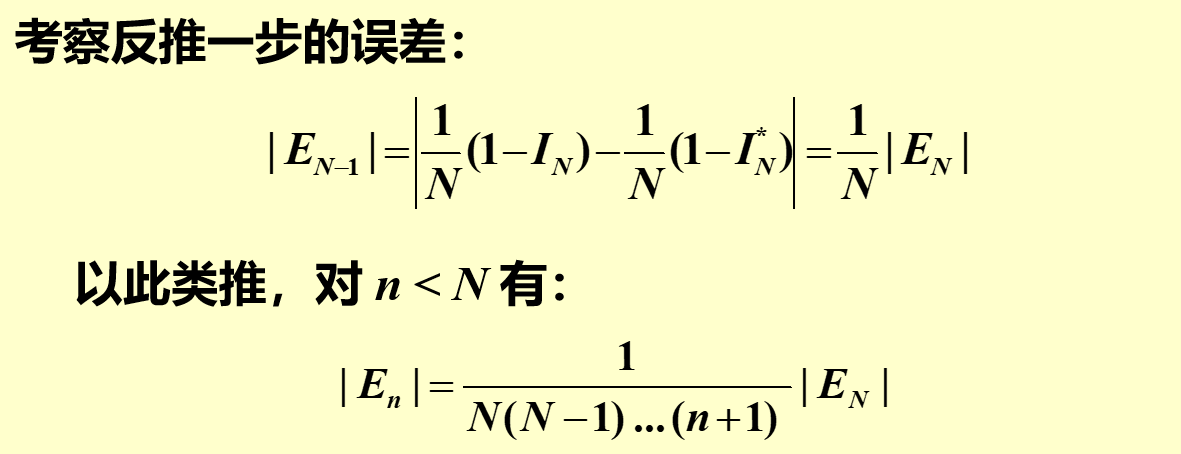
\includegraphics[width=0.7\linewidth]{image/误差3}
 	\caption{稳定算法}
 	\label{fig:3}
 \end{figure}
\begin{table}[h]
	\centering
	\caption{两种方法与标准值的比较}
	\begin{tabular}{cccccc}
		\toprule
		\(N\) & 标准值 \(y_{\text{ref}}\) & 方法1结果 \(y_1\) & 方法2结果 \(y_2\) & 方法1相对误差 & 方法2相对误差 \\ 
		\midrule
		\(0\)    & 0.632120559     & 0.63212056     & 0.63212056     & \(1.58 \times 10^{-6}\%\) & \(1.58 \times 10^{-6}\%\) \\
		\(1\)    & 0.367879441     & 0.36787944     & 0.36787944     & \(2.72 \times 10^{-6}\%\) & \(2.72 \times 10^{-6}\%\) \\
		\(2\)    & 0.264241118     & 0.26424112     & 0.26424112     & \(7.57 \times 10^{-6}\%\) & \(7.57 \times 10^{-6}\%\) \\
		\(3\)    & 0.207276647     & 0.20727664     & 0.20727665     & \(3.38 \times 10^{-6}\%\) & \(1.45 \times 10^{-5}\%\) \\
		\(4\)    & 0.170893412     & 0.17089344     & 0.17089341     & \(1.64 \times 10^{-5}\%\) & \(1.17 \times 10^{-5}\%\) \\
		\(5\)    & 0.145532941     & 0.1455328     & 0.14553294     & \(0.097\% \) & \(6.87 \times 10^{-6}\%\) \\
		\(6\)    & 0.126802357     & 0.1268032     & 0.12680236     & \(0.66\% \) & \(2.36 \times 10^{-5}\%\) \\
		\(7\)    & 0.112383504     & 0.1123776     & 0.11238350     & \(0.0053\% \) & \(3.55 \times 10^{-5}\%\) \\
		\(8\)    & 0.100931967     & 0.1009792     & 0.10093197     & \(0.047\% \) & \(2.82 \times 10^{-6}\%\) \\
		\(9\)    & 0.091612293     & 0.0911872     & 0.09161229     & \(0.46\% \) & \(3.38 \times 10^{-6}\%\) \\
		\(10\)    & 0.0838770701    & 0.088128     & 0.08387707    & \(5.07\% \) & \(1.19 \times 10^{-5}\%\) \\
		\(11\)    & 0.0773522289    & 0.030592     & 0.07735225    & \(60.5\% \) & \(2.66 \times 10^{-4}\%\) \\
		\(12\)    & 0.0717732536    & 0.632896     & 0.07177296    & \(782\% \) & \(4.01 \times 10^{-4}\%\) \\
		\(13\)    & 0.0669477026    & -7.227648    & 0.06695156    & \(10800\% \) & \(0.0056\% \) \\
		\(14\)    & 0.0627321639    & 102.187072   & 0.06267811    & \(162900\% \) & \(0.084\% \) \\
		\(15\)    & 0.0590175409    & -1531.80608  & 0.05982836    & \(2.60 \times 10^6\% \) & \(1.35\% \) \\
		\bottomrule
	\end{tabular}
\end{table}
 两种方法对比, 可以看到方法1即使初始误差较小, 也会快速积累; 方法2在$N$较大估计一个初值, 倒推误差快速缩小. 方法2, 求$I_{15}$, 取$I_{20}^*=\dfrac{1}{2}[\dfrac{1}{e\cdot21}+\dfrac{1}{21}]\approx 0.03256855812$, 递推得到$I_{15}\approx 0.05901754785$, 相对误差\(1.18 \times 10^{-5}\%\).
 
 \begin{remark}
 	在数值计算中,算法的\textbf{数值稳定性}对结果的准确性至关重要。本文通过计算积分递推公式\[ I_n=1-nI_{n-1},I_0=1-e^{-1} \]发现即使采用双精度浮点运算(MATLAB 或 Python 默认计算方式),由于舍入误差的累积和放大,显著偏差的计算结果只是推迟但仍会出现(如$I_{18}=-0.0294536708$, 理论值应为严格正数). 即使采用高精度算术, 不稳定的算法仍会导致结果失效.
 \end{remark}
\section{误差与有效数字}

\begin{itemize}
	\item \textbf{绝对误差}: $e^*=x^*-x$, 其中$x$为精确值,$x^*$为$x$的近似值.
	\item $|e^*|$的上限记为$\varepsilon^*$, 称为\textbf{绝对误差限}.
	\item \textbf{相对误差}: $e^*_r=\dfrac{e^*}{x}$
	\item \textbf{相对误差上限}定义为: $\varepsilon^*_r=\dfrac{\varepsilon^*}{|x^*|}$, 注意分母使用的是近似值$x^*$, 在合理的情况下反映了数量级.
\end{itemize}
\begin{definition}
	若近似值$x^*$的误差限是某一位的半个单位, 该位到$x^*$的第一位非零数字共有$n$位, 则$x^*$有$n$位有效数字.
\end{definition}

用科学计数法, 记$x^*=\pm0.a_1a_2\cdots a_n\times10^m(a_1\neq0)$, 若$|x-x^*|<0.5\times10^{m-n}$, 则称$x^*$有$n$位有效数字.
\begin{figure}[H]
	\centering
	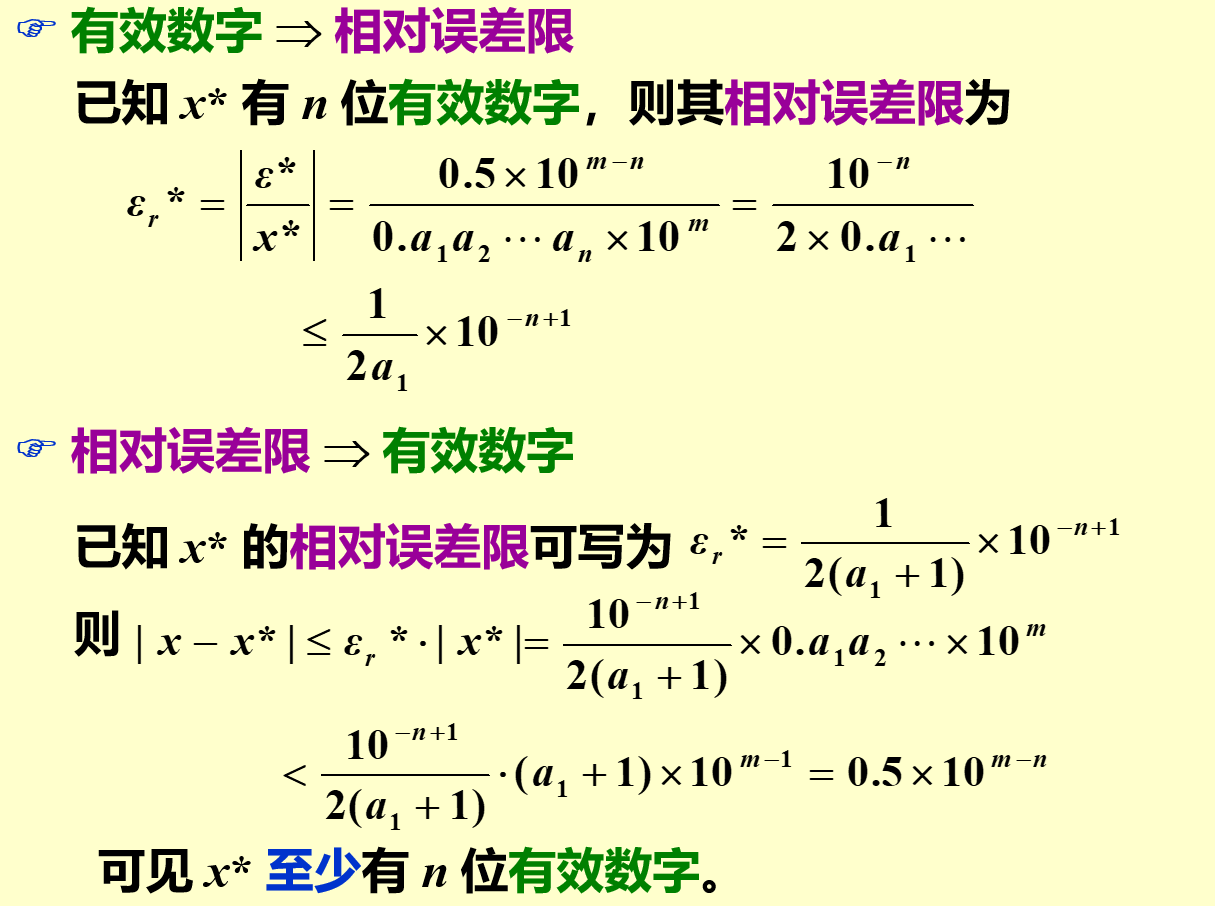
\includegraphics[width=0.7\linewidth]{image/误差5}
	\caption{有效数字与相对误差的关系}
	\label{fig:5}
\end{figure}
\section{函数的误差估计}
问题:对于$A=f(x)$, 若用$x^*$取代$x$, 将对$A$产生什么影响?
\begin{figure}[H]
	\centering
	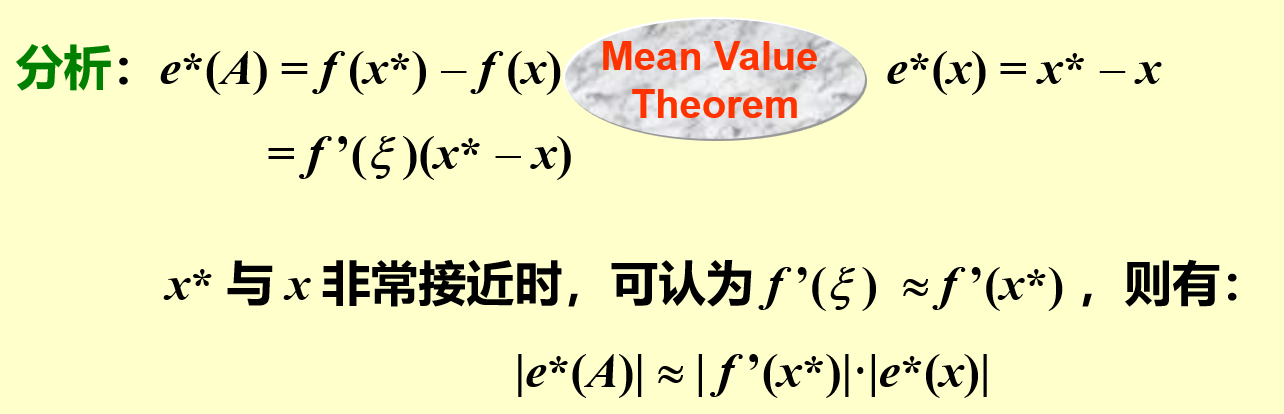
\includegraphics[width=0.8\linewidth]{image/误差6}
	\caption{函数的误差估计1}
	\label{fig:6}
\end{figure}
即: $x^*$产生的误差经过$f$作用后被放大/缩小了$|f'(x^*)|$倍. 故称$|f'(x^*)|$为放大因子或绝对条件数.而
\begin{figure}[H]
	\centering
	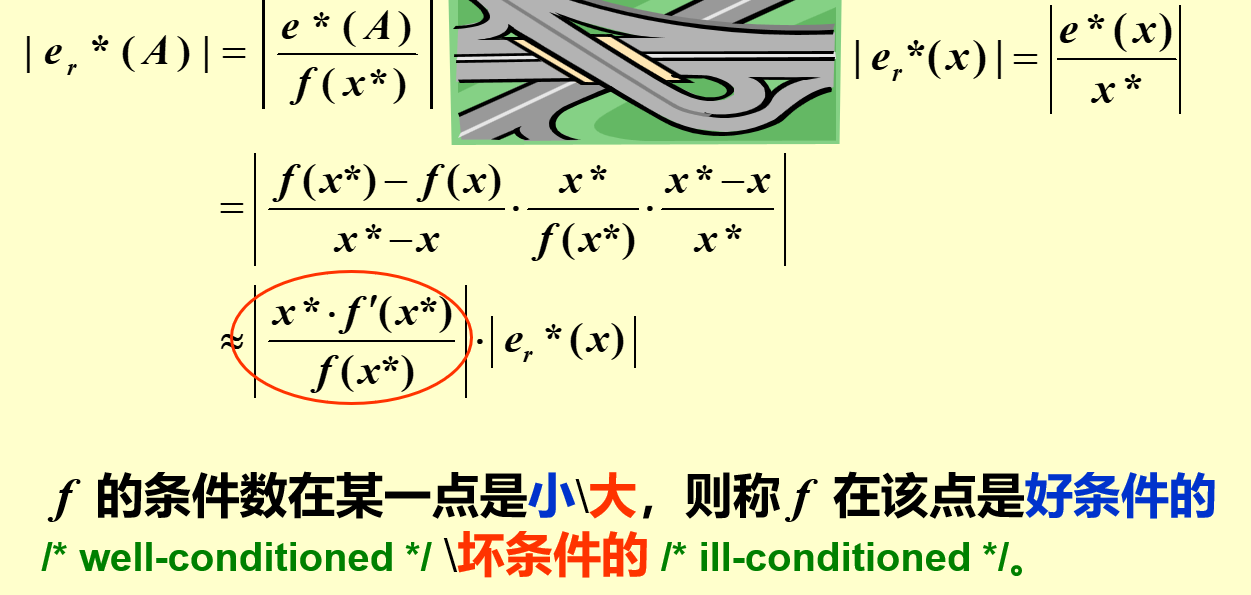
\includegraphics[width=0.8\linewidth]{image/误差7}
	\caption{函数的误差估计2}
	\label{fig:7}
\end{figure}
\section{几点注意事项}
\begin{itemize}
	\item 避免相近二数直接相减, 可能减少有效数字位数
	\begin{figure}[H]
		\centering
		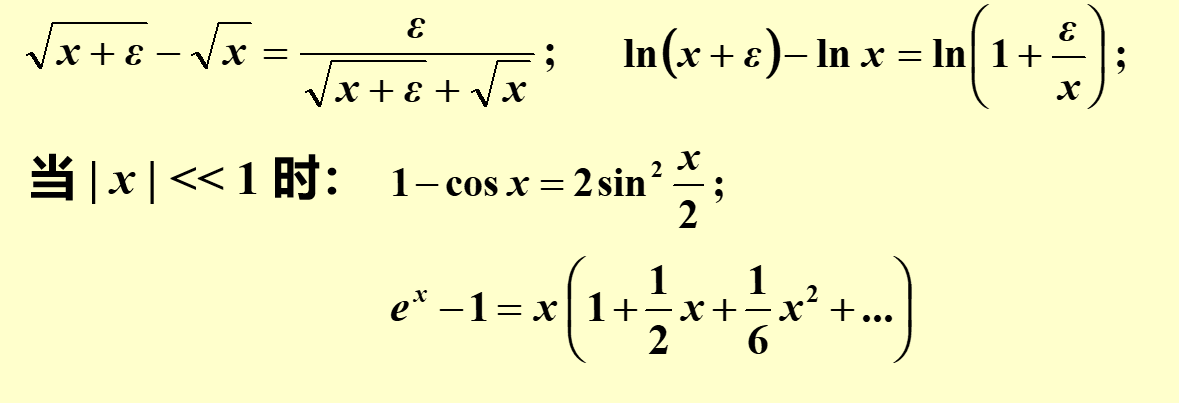
\includegraphics[width=0.9\linewidth]{image/误差4}
		\caption{几种经验性避免方法}
		\label{fig:4}
	\end{figure}
	\item 避免小分母 :  分母小会造成浮点精度不足;
	\item 避免大数吃小数导致浮点数精度问题;
	\item 先化简再计算,减少步骤,避免误差积累;
	\item 选用稳定的算法.
\end{itemize}
\section{思考题与习题}
\chapter{函数逼近与快速傅里叶变换}
这一章存在一个典型问题, 就是大多数非数学专业的人本科并没有学线性空间, 也不理解线性代数怎么与多项式有关系了, 因此就学的云里雾里.

已知$x_1,\cdots,x_N;y_1,\cdots,y_N$, 第二章有插值法求得近似函数$P(x)\approx f(x)$, 但是N很大超过拟合需要的点数目, 并且$y_i$本身是不准确的测量值, 插值法将误差完全包含进拟合函数. 此时没必要使用插值, 而应该拟合逼近, 例如最小二乘拟合.
\section{函数逼近的基本概念}
$\sin x-\dfrac{x^2}{2}=0$在(0,1)内的根的近似值($\zeta=0.4*10^{-5}$)
\chapter{非线性方程与方程组的数值解法}
为什么方程需要数值解法?首先$n$次代数方程$n$个根, $n\ge 5$时没有求根公式, $n=3,\,4$时求根公式也比较复杂; 其次包含对数函数、指数函数、三角函数等超越函数的超越方程本身大多没有解析解.
\section{方程求根与二分法}
二分法的原理高中就学过, 但是不能用计算器所以高中不会考, 在此熟悉步骤.

零点定理: 在$[a,b]$连续且$f(a)f(b)<0$, 则说明在$(a,b)$至少有一个实根, 称$[a,b]$为方程的\textbf{有根区间}, 但没有确定数目, 配合单调性可以确定根的唯一性. 



二分法的思想是将有根区间折半进行搜索, 即对有根区间$[a,b]$,取中点$x=\frac{a+b}{2}$将它分为两半,检查$f(x_1)$
与$f(a)$是否同号,如果确系同号,说明所求的根$x^*$在$x_1$的右侧,这时令$a_1=x_1,\,b_1,=b$; 否则$x^*$必在$x_1$的左侧,这时令$a_1=a,\,b_1=x_1$, 不管出现哪一种情况,新的有根区间仅
为原来的一半.


设置终止条件$|x_{k+1}-x_k|<\varepsilon_1$或$|f(x)|<\varepsilon_2$, 但是不能保证x的精度.
\section{习题}
\begin{exercise}
	用二分法求方程$x^2-x-1=0$的正根, 要求误差小于0.05.
\end{exercise}
解: 设$f(x)=x^2-x-1$, 得到$f^{'}(x)=2x-1$, 在$(0,\dfrac{1}{2})<0$, $(\dfrac{1}{2},+)>0$
\section{计算实习题}
\begin{exercise}
	用二分法求方程$x^2-x-1=0$的正根, 要求误差小于0.05.
\end{exercise}
\chapter{非线性方程(组)的数值解法}

\chapter{线性方程组的数值解法}

\chapter{插值方法与数值逼近}
\chapter{数值积分}
\chapter{矩阵特征值与特征向量的计算}
\chapter{常微分方程初值问题的数值解法}
\section{习题}
\begin{exercise}
	利用四阶经典的龙格-库塔法求解初边值问题\[ 
	\begin{cases}
		y'+y=0\\
		y(0)=1
	\end{cases}
	\]
	讨论步长h应取何值方能保证方法的绝对稳定性?取步长$h=0.2$,求$x=0.2$, $x=0.4$时的数值解,要求写出由$h$,$x_n$,$y_n$直接计算的迭代公式(计算过程中保留小数点后3位).
\end{exercise}
\begin{solution}
	\noindent\textbf{1. 写出微分方程与经典四阶龙格-库塔公式}
	
	原方程:$y' = -y = f(x, y)$,初值 $y(0) = 1$。
	
	经典四阶龙格-库塔公式:
	\[
	\begin{cases}
		k_1 = f(x_n, y_n), \\
		k_2 = f\left(x_n + \frac{h}{2}, y_n + \frac{h}{2}k_1\right), \\
		k_3 = f\left(x_n + \frac{h}{2}, y_n + \frac{h}{2}k_2\right), \\
		k_4 = f\left(x_n + h, y_n + h k_3\right), \\
		y_{n+1} = y_n + \frac{h}{6}(k_1 + 2k_2 + 2k_3 + k_4).
	\end{cases}
	\]
	
	代入 $f(x, y) = -y$:
	\[
	\begin{aligned}
		k_1 &= -y_n, \\
		k_2 &= -\left(y_n + \frac{h}{2}k_1\right) = -y_n\left(1 - \frac{h}{2}\right), \\
		k_3 &= -\left(y_n + \frac{h}{2}k_2\right) = -y_n\left[1 - \frac{h}{2} + \frac{h^2}{4}\right], \\
		k_4 &= -\left(y_n + h k_3\right) = -y_n\left[1 - h + \frac{h^2}{2} - \frac{h^3}{4}\right].
	\end{aligned}
	\]
	
	代入 $y_{n+1}$ 公式:
	\[
	\begin{aligned}
		y_{n+1} &= y_n + \frac{h}{6}\left[k_1 + 2k_2 + 2k_3 + k_4\right] \\
		&= y_n - \frac{h y_n}{6}\left[1 + 2\left(1 - \frac{h}{2}\right) + 2\left(1 - \frac{h}{2} + \frac{h^2}{4}\right) + \left(1 - h + \frac{h^2}{2} - \frac{h^3}{4}\right)\right].
	\end{aligned}
	\]
	
	计算括号内:
	\[
	1 + 2 + 2 + 1 = 6, \quad
	- h - h - h = -3h, \quad
	\frac{h^2}{2} + \frac{h^2}{2} = h^2, \quad
	- \frac{h^3}{4}.
	\]
	所以:
	\[
	y_{n+1} = y_n\left[1 - h + \frac{h^2}{2} - \frac{h^3}{6} + \frac{h^4}{24}\right].
	\]
	记
	\[
	R(h) = 1 - h + \frac{h^2}{2} - \frac{h^3}{6} + \frac{h^4}{24}.
	\]
	则迭代公式为:
	\[
	y_{n+1} = R(h) \cdot y_n.
	\]
	
	\noindent\textbf{2. 绝对稳定性条件}
	
	绝对稳定性要求 $|R(h)| < 1$。对于 $h > 0$,$R(h)$ 是 $e^{-h}$ 的四阶泰勒展开,单调递减。当 $h$ 增大到使 $R(h) < -1$ 时失稳。
	
	经典四阶 R-K 法的绝对稳定区间(对 $y' = \lambda y$,$\mathrm{Re}(\lambda) < 0$)满足:
	\[
	h|\lambda| \le 2.785293\ldots
	\]
	这里 $\lambda = -1$,所以:
	\[
	h < 2.785
	\]
	可保证绝对稳定性。
	
	\noindent\textbf{3. 取 $h=0.2$ 计算数值解}
	
	\[
	R(0.2) = 1 - 0.2 + \frac{0.04}{2} - \frac{0.008}{6} + \frac{0.0016}{24}
	\]
	逐步计算(保留小数点后 6 位用于中间过程):
	\[
	\begin{aligned}
		&1 - 0.2 = 0.8, \\
		&0.8 + 0.02 = 0.82, \\
		&0.82 - 0.001333 = 0.818667, \\
		&0.818667 + 0.000067 = 0.818734.
	\end{aligned}
	\]
	所以:
	\[
	y_{n+1} = 0.818734 \cdot y_n.
	\]
	
	$y_0 = 1$:
	\[
	y(0.2) \approx y_1 = 0.818734 \approx 0.819 \quad (\text{保留 3 位}),
	\]
	\[
	y(0.4) \approx y_2 = 0.818734 \times 0.818734 \approx 0.670312 \approx 0.670 \quad (\text{保留 3 位}).
	\]
	
	\noindent\textbf{最终答案:}
	\[
	\boxed{0.819, \ 0.670}
	\]
	绝对稳定性要求步长 $h < 2.785$。
\end{solution}
\end{document}
